% -*- mode: latex; mode: auto-fill; coding: utf-8; -*-


\label{sec:applying-fem}
In this section, we follow the seven step procedure of creating a
discrete finite element model introduced in section
\vref{sec:using-the-FEM}.
%
To summarize we have chosen the following which will be further
elaborated in upcoming sections. At step four, assembling the system
equations, no choice can be made so our choices are listed three steps
at the time.
%
We discretize the solution region into four-node tetrahedral elements,
select linear volumetric coordinates as our interpolation
functions, and use elasticity theory and energy preservation to
describe the element properties.
%
At this point we assemble the element properties to obtain the system
equations precisely as described in section
\vref{sec:asseble-the-element-properties}.
%
Then we impose boundary conditions by fixing nodal positions, and
construct an equation solver using the Total Lagrangian Explicit
Dynamics technique. Lastly we add fracture mechanics as additional
computations.

\section{Discretize the Continuum}
The continuum is a volumetric body. Therefore we need an element type
which covers a volume. We have chosen the four-node tetrahedron, as this
is the simplest volumetric element and because it is the most commonly
used three-dimensional element type.

\begin{figure}
  \centering
  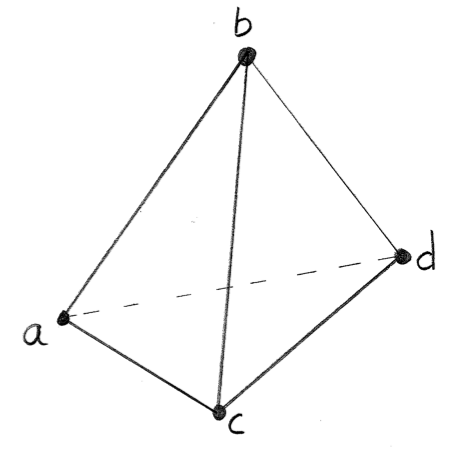
\includegraphics[width=4cm]{./images/finite_element_method_tetrahedron.png}
\caption{Four-node tetrahedron nodes with node names.}
\label{fig:tetrahedron}
\end{figure}

The four-node tetrahedron element has 4 nodes, 4 faces and 6 edges.
For a tetrahedron with vertices: $a,b,c,d$, as illustrated in figure
\vref{fig:tetrahedron}, the nodes are named according to the following
rule: If a tetrahedron is defined in a right-hand
Cartesian coordinate system, the nodes are named so that nodes $a$,
$b$, $c$ are ordered counterclockwise when viewed from node $d$. By
naming the nodes this way we ensure that the following equation for
calculating the volume always gives a positive value.
\citebook{page~159}{book:fem-engineers}.
%
The volume is then calculated as:

\begin{equation}
    V = \frac {|(a-d) \cdot ((b-d) \times (c-d))|}{6}. 
\end{equation}

% Later, in section \vref{}, we will see that it will be necessary to be
% able to compare the length of the tetrahedrons edges and angles
% within a tetrahedron.
% The angle between two sides in a tetrahedron
% (planes) is in geometry called their dihedral angle.

% \begin{figure}
%   \centering
%   \includegraphics[width=5cm]{./images/google-dihedral-angle.png}
% \caption{Dihedral angle}
% \label{fig:dihedral-angle}
% \end{figure}

% The dihedral angle between the two planes, at their intersection line, is
% the angle between the two planes' normal vectors and can be calculated by:

% \begin{equation}
%   \cos \angle_{\alpha \beta} = n_{\alpha} \cdot n_{\beta}
% \end{equation}

Tetrahedron structures gives good approximations to the continuum
body. As it is hard to imagine how tetrahedra fill a body
figure \vref{fig:hexahedron2tetrahedra} gives an example of how a
box can be fully covered by five tetrahedra, which is the minimum
number nessecary to fill a box.

\begin{figure}
  \centering
  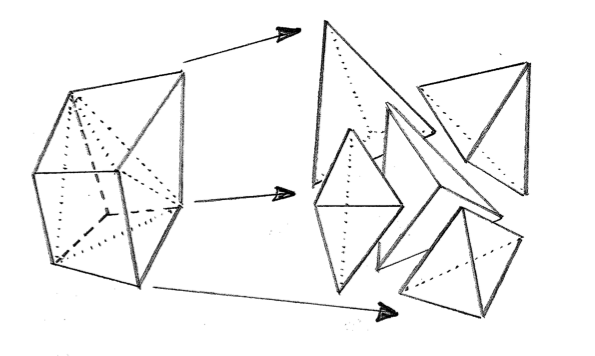
\includegraphics[width=12cm]{./images/finite_element_method_hexahedron2tetrahedra.png}
\caption{A general hexahedron decomposed into five tetrahedra.}
\label{fig:hexahedron2tetrahedra}
\end{figure}
%figure from: fem-engineers, p. 143

As in the case of approximating a curve with triangular elements in
section \vref{sec:discretize-the-continuum}, when a larger amount of
geometrically smaller elements are used, we get a higher accuracy on
the curve approximation.

\section{Selecting the Interpolation Functions}
\label{sec:the-interpolation-functions-we-have-chosen}
As interpolation functions we use the volumetric coordinates as described
in section \vref{sec:natural-coordinates-3d}.
% downwards rewritten from p 163
We have chosen natural coordinates as interpolation functions by
setting the interpolation functions equal to the natural
coordinates.

\begin{equation}
N_i(x,y,z) = L_i(x,y,z)
\end{equation}
% upwards rewritten from p 163

The unknown field variable is in our case the displacements. We have a
three component displacement vector at each of the four nodes, as
illustrated in figure \vref{fig:displacement-vectors}, giving a total
of 12 displacement variables.
 
\begin{figure}
  \centering
  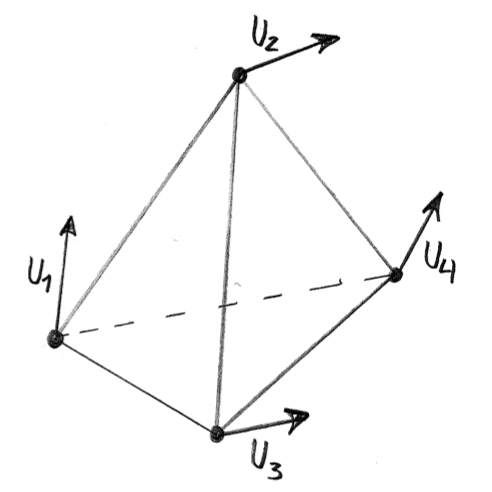
\includegraphics[width=4cm]{./images/finite_element_method_displacement_vectors.png}
\caption{Displacement vectors in an four-node tetrahedron element.}
\label{fig:displacement-vectors}
\end{figure}

The interpolation functions for our model define the element-wise
displacement functions by interpolating the four nodal displacement
vectors, with their 12 variables over the element. The 12 values are
represented by $U$, where the right superscript denoted the node
number and the right subscript the axial direction.

\begin{equation}
U^T = \left[
\begin{array}{cccccccccccc}
u^{1}_x & u^{1}_y & u^{1}_z & 
u^{2}_x & u^{2}_y & u^{2}_z &
u^{3}_x & u^{3}_y & u^{3}_z & 
u^{4}_x & u^{4}_y & u^{4}_z 
\end{array}
\right]
\end{equation}

and hence the continuous function $U(x,y,y) = N U$ where $N$, called the
\defit{interpolation matrix}, is defined by

\begin{equation}
\label{eq:interpolation_matrix}
N = \left[
\begin{array}{cccccccccccc}
N_1 & 0 & 0 & N_2 & 0 & 0 & N_3 & 0 & 0 & N_4 & 0 & 0 \\
0 & N_1 & 0 & 0 & N_2 & 0 & 0 & N_3 & 0 & 0 & N_4 & 0 \\
0 & 0 & N_1 & 0 & 0 & N_2 & 0 & 0 & N_3 & 0 & 0 & N_4
\end{array}
\right]
\end{equation}

which gives the displacement functions
\citebook{page~262}{book:fem-engineers}:

\begin{equation}
U(x,y,z) =
\begin{Bmatrix}
U_x(x,y,z) 
\vspace{2mm} \\
U_y(x,y,z) 
\vspace{2mm} \\
U_z(x,y,z)
\end{Bmatrix}
= N U =
\begin{Bmatrix}
  L_1(x,y,z) U_x^{1} + L_2(x,y,z) U_x^{2}
  + L_3(x,y,z) U_x^{3} + L_4(x,y,z) U_x^{4}
\vspace{2mm}\\
  L_1(x,y,z) U_y^{1} + L_2(x,y,z) U_y^{2}
  + L_3(x,y,z) U_y^{3} + L_4(x,y,z) U_y^{4} 
\vspace{2mm}\\
  L_1(x,y,z) U_z^{1} + L_2(x,y,z) U_z^{2} 
  + L_3(x,y,z) U_z^{3} + L_4(x,y,z) U_z^{4}
\end{Bmatrix}
\end{equation}

where $L_i$ is given by equation \eqref{eq:li}.

\section{Finding the Element Properties}
%going ... to describe the relation of external forces and nodal
%displacement via the potential energy of these quantities
%
To determine the element properties we are going to use the elasticity
theory discussed in section \vref{sec:elasticity}. The element
properties are related as follows:
displacement to strain, stress to strain via the theory of
elasticity, and finally we convert stress and strain into potential
energy. The goal in this section, is to construct a function
that describes the potential energy of an element in terms of its nodal
displacements $U$. The equation for potential energy is defined
to be the potential energy of the work done by the external forces
($E_V$) and the internal strain energy ($E_S$).

\begin{equation}
\prod (x,y,z) = E_S + E_V = E_S - W
\end{equation}

%Where $E_S$ is the strain energy and $E_V$ is the potential energy of
%the external forces.
Where $E_V = -W$ is defined in equation
\eqref{eq:EW} on page \pageref{eq:EW}. From equation
\eqref{eq:strain_energy} and \eqref{eq:external-work} we have that:

\begin{equation*}
E_S =  \int_V \varepsilon \cdot \sigma \ dV
+ \int_V \gamma \cdot \tau \ dV
\qquad \qquad E_V = - W = - \int_V u \cdot f \ dV
\end{equation*}

Instead of using the dot product notation we will use transposed
matrices from here on. Furthermore, the four $3 \times 1$ vectors,
stress ($\sigma$ and $\tau$) and strain ($\varepsilon$ and $\gamma$),
have been combined into two $6 \times 1$ vectors, and use the per
element displacement and force vectors $U$ and $F$, which look like
this:

\begin{equation}
\prod (x,y,z) =  \int_V 
\begin{Bmatrix}
\varepsilon \\
\gamma
\end{Bmatrix}
^T
\begin{Bmatrix}
\sigma \\
\tau
\end{Bmatrix}
dV - \int_V U^T F \ dV
\end{equation}

As $E_V$ is already a function of $u$, we concentrate on $E_S$.
The material matrix $C$ from the elasticity theory relates
stress to strain. Appendix \ref{appendix:hookes-law-on-matrix-form}
defines this material matrix and the matrix relation between stress
and strain, repeated below for convenience:

\begin{equation*}
\begin{Bmatrix}
\sigma \\
\tau
\end{Bmatrix}
= C 
\begin{Bmatrix}
\varepsilon \\
\gamma
\end{Bmatrix}
\end{equation*}

\begin{equation}
E_S (x,y,z) = \int_V 
\begin{Bmatrix}
\varepsilon \\
\gamma
\end{Bmatrix}
^T
\begin{Bmatrix}
\sigma \\
\tau
\end{Bmatrix}
dV = \int_V
\begin{Bmatrix}
\varepsilon \\
\gamma
\end{Bmatrix}
^T C
\begin{Bmatrix}
\varepsilon \\
\gamma
\end{Bmatrix}
dV
\end{equation}

The final step is a little more complicated, here we will relate
strain to displacement. Recalling from section
\vref{sec:physics_strain} that normal strain is defined by equation
\eqref{eq:individual-normal-strain} as:

\begin{equation*}
\varepsilon_x = \frac{\partial u_x}{\partial x} \hspace{10 mm}
\varepsilon_y = \frac{\partial u_y}{\partial y} \hspace{10 mm}
\varepsilon_z = \frac{\partial u_z}{\partial z}
\end{equation*}

and shearing strain by equation \eqref{eq:individual-shear-strain} as:

\begin{equation*}
  \gamma_{xy} = \frac{\partial u_x}{\partial y} +
  \frac{\partial u_y}{\partial x} \hspace{10 mm}
  \gamma_{xz} = \frac{\partial u_x}{\partial z} +
  \frac{\partial u_z}{\partial x} \hspace{10 mm}
  \gamma_{yz} = \frac{\partial u_y}{\partial z} +
  \frac{\partial u_z}{\partial y}
\end{equation*}

On matrix form this looks like the following:

\begin{equation}
\begin{Bmatrix}
\varepsilon \\
\gamma
\end{Bmatrix}
= 
\begin{Bmatrix}
\varepsilon_x \\
\varepsilon_y \\
\varepsilon_z \\
\gamma_{xy} \\
\gamma_{xz} \\
\gamma_{yz}
\end{Bmatrix}
= L U(x,y,z) = L N U = B U
\end{equation}

where the \defit{differential operator} $L$ is defined as
\citebook{page~233}{book:fem-engineers}:

\begin{equation}
L =
\begin{bmatrix}
\frac{\partial}{\partial x} & 0 & 0 \\
\vspace{2mm}
0 & \frac{\partial}{\partial y} & 0 \\
\vspace{2mm}
0 & 0 & \frac{\partial}{\partial z} \\
\vspace{2mm}
\frac{\partial}{\partial y} & \frac{\partial}{\partial x}  & 0 \\
\vspace{2mm}
\frac{\partial}{\partial z} & 0 & \frac{\partial}{\partial x} \\ 
\vspace{2mm}
0 & \frac{\partial}{\partial z}  & \frac{\partial}{\partial y}
\end{bmatrix}
\end{equation}

\layoutnewpage

and the \defit{strain interpolation matrix} $B$
\citebook{page~235}{book:fem-engineers}:

\begin{equation}
\label{eq:strain_interpolation_matrix}
\begin{aligned}
B &= L N = \left[
\begin{array}{cccccccccccc}
  \frac{\partial N_1}{\partial x} & 0 & 0 &
  \frac{\partial N_2}{\partial x} & 0 & 0 &
  \frac{\partial N_3}{\partial x} & 0 & 0 &
  \frac{\partial N_4}{\partial x} & 0 & 0 \\
\vspace{2mm}
  0 & \frac{\partial N_1}{\partial y} & 0 &
  0 & \frac{\partial N_2}{\partial y} & 0 &
  0 & \frac{\partial N_3}{\partial y} & 0 &
  0 & \frac{\partial N_4}{\partial y} & 0 \\
\vspace{2mm}
  0 & 0 & \frac{\partial N_1}{\partial z} &
  0 & 0 & \frac{\partial N_2}{\partial z} &
  0 & 0 & \frac{\partial N_3}{\partial z} &
  0 & 0 & \frac{\partial N_4}{\partial z} \\
\vspace{2mm}
  \frac{\partial N_1}{\partial y} & \frac{\partial N_1}{\partial x}  & 0 &
  \frac{\partial N_2}{\partial y} & \frac{\partial N_2}{\partial x}  & 0 &
  \frac{\partial N_3}{\partial y} & \frac{\partial N_3}{\partial x}  & 0 &
  \frac{\partial N_4}{\partial y} & \frac{\partial N_4}{\partial x}  & 0 \\
\vspace{2mm}
  \frac{\partial N_1}{\partial z} & 0 & \frac{\partial N_1}{\partial x} &
  \frac{\partial N_2}{\partial z} & 0 & \frac{\partial N_2}{\partial x} &
  \frac{\partial N_3}{\partial z} & 0 & \frac{\partial N_3}{\partial x} &
  \frac{\partial N_4}{\partial z} & 0 & \frac{\partial N_4}{\partial x} \\
\vspace{2mm}
  0 & \frac{\partial N_1}{\partial z} & \frac{\partial N_1}{\partial y} &
  0 & \frac{\partial N_2}{\partial z} & \frac{\partial N_2}{\partial y} &
  0 & \frac{\partial N_3}{\partial z} & \frac{\partial N_3}{\partial y} &
  0 & \frac{\partial N_4}{\partial z} & \frac{\partial N_4}{\partial y}
\end{array}
\right] \\ \\
& \hspace{4mm} = \frac{1}{6V} \left[
\begin{array}{cccccccccccc} 
b_1 & 0 & 0 &
b_2 & 0 & 0 &
b_3 & 0 & 0 &
b_4 & 0 & 0 \\

0 & c_1 & 0 &
0 & c_2 & 0 &
0 & c_3 & 0 &
0 & c_4 & 0 \\

0 & 0 & d_1 &
0 & 0 & d_2 &
0 & 0 & d_3 &
0 & 0 & d_4 \\

c_1 & b_1 & 0 &
c_2 & b_2 & 0 &
c_3 & b_3 & 0 &
c_4 & b_4 & 0 \\

d_1 & 0 & b_1 &
d_2 & 0 & b_2 &
d_3 & 0 & b_3 &
d_4 & 0 & b_4 \\

0 & d_1 & c_1 &
0 & d_2 & c_2 &
0 & d_3 & c_3 &
0 & d_4 & c_4 
\end{array}
\right]
\end{aligned}
\end{equation}

Returning to the equation for strain energy we have:

\begin{equation}
E_S (x,y,z)
= \int_V
\begin{Bmatrix}
\varepsilon \\
\gamma
\end{Bmatrix}
^T C
\begin{Bmatrix}
\varepsilon \\
\gamma
\end{Bmatrix}
dV = \int_V U^T N^T L^T C L N U \ dV
= \int_V U^T B^T C B U \ dV
\end{equation}

and because the integral over the volume $V$ only includes constant
terms \citebook{page~263}{book:fem-engineers}:

\begin{equation}
\begin{aligned}
E_S (x,y,z) 
&= \int_V U^T B^T C B U \ dV 
= U^T B^T C B U \int_V dV \\
&= U^T B^T C B U V 
= U^T V B^T C B U
\end{aligned}
\end{equation}

now defining the stiffness matrix to be:

\begin{equation}
K^{(e)} = V B^T C B
\end{equation}

the function becomes:

\begin{equation}
E_S (x,y,z) = U^T K U
\end{equation}

Inserting this into the function for potential energy and solving
the integration of external force as above, gives:

\begin{equation}
\label{eq:linear-sys-eq}
\prod (x,y,z) = E_S(x,y,z) - U^T F \int_V dV = U^T K U - U^T F V
\end{equation}

To get an impression and overview of the equation sizes we list the
matrix sizes: $U$: $12 \times 1$, $F$: $12 \times 1$, $C$: $6 \times
6$, $L$: $6 \times 3$, $N$: $3 \times 12$,
$B$: $6 \times 12$, and finally $K$: $12 \times 12$.

%formulas from: \citebook{page~233}{book:fem-engineers}.
%formulas from: \citebook{page~227}{book:fem-engineers}.
%formulas from: \citebook{page~229-230}{book:fem-engineers}.
%formulas from: 
% fem pages: 227, 233, 234, 263, 659, 661, 666

\section{Assembling the System Equations}
The system equations are assembled in a straightforward manner. We
expand the element stiffness matrices and add them to yield the system
stiffness matrix as illustrated by the example in section
\vref{sec:example-of-two-tetrahedrons}.
To get an idea of the size of the complete system we consider a system
with 100 four-node tetrahedron elements, with 70 global nodes. The size
of the complete system will then have a force vector $F$: $70 \times
1$ and $U$: $70 \times 1$. The stiffness matrix for the system will
then be $70 \times 70$ in size.
%
The example above is relatively small compared with the models we are
using. The number of elements in our models range from 1000 to 10000
elements.
%
%As we shall see later we use an explicit solver which means that
%the complete system matrix never has to be assembled when performing
%the actual calculations.

%265 sum N - i,j,k

\section{Imposing the Boundary Conditions}
Because the number of unknowns in the system are larger that then
number of equations, we need to impose boundary conditions, so it is
possible to solve the system.
%
Recall that we aim at modelling fragmentation of a tooth, as part of
the surgical procedure of removing a wisdom tooth. In this scenario 
a part of the tooth is located in the jaw, which effectively restrains
the position of its roots.
%
By fixing the position of nodes located in the jaw, we impose a
boundary condition hereby restricting the solution domain.

\section{Solving the System Equations}
To solve the system equations we need to use the principle of minimum
potential energy. To find this minimum potential energy the system
equations have to be differentiated \citebook{page~85-87}{book:bathe}.

% \begin{equation}
% \partial \prod (x,y,z) = 0
% \end{equation}

% where each spatial component of the equation can be calculated
% separately and summed.

% \begin{equation}
% \label{eq:partial-energy}
% \partial \prod (x,y,z) =
% \frac{\partial \prod}{ \partial x} +
% \frac{\partial \prod}{ \partial y} +
% \frac{\partial \prod}{ \partial z}
% \end{equation}

% Therefore we can rephrase equation \eqref{eq:partial-energy} into
% its spatial component \citebook{page~119-120}{book:bathe}.

\begin{equation}
\label{eq:dp-eq-zero}
\frac{\partial \prod}{ \partial x} = 0
\qquad
\frac{\partial \prod}{ \partial y} = 0
\qquad
\frac{\partial \prod}{ \partial z} = 0
\end{equation}

in our case, repeated from equation \eqref{eq:linear-sys-eq}:

\begin{equation*}
\prod (x,y,z) = U^T K U - U^T F V
\end{equation*}

by applying equation \eqref{eq:dp-eq-zero} this becomes:

\begin{equation}
\partial \prod (x,y,z) = K U - F = 0
\end{equation}

which in turn can be stated as:

\begin{equation}
\label{eq:std-fem-eq}
K U = F
\end{equation}

%an equation with this appearance is sed
This equation relates displacements to external forces via the
stiffness matrix. The stiffness matrix describes physical laws of the
problem we are modelling. The stiffness matrix could model any
problem, making this equation general. Therefore equation
\eqref{eq:std-fem-eq} is called the
\defit{standard finite element equation}.

\subsection{Introducing Time Into the Equation}
Equation \eqref{eq:std-fem-eq} defines the standard finite element
equation of equilibrium but only for static problems. In dynamic
problems we need to introduce time into the equation.
%
The most important equation in dynamic problems is based
upon the static case as defined in equation \eqref{eq:std-fem-eq} but now there
is motion. According to Newton's second law motion is introduced as mass times
acceleration. By introducing this into the equation we obtain 

\begin{equation}
\label{eq:undamped_harmonic_motion}
M \ddot{U} + K U = F
\end{equation}
  
where $M$ is the mass matrix, the dot notation is used for
time derivatives so $\ddot{U}$ is the acceleration equal
to the second derivative of the displacement, $K$ is the stiffness
matrix and $U$ is the displacement vector. Equation
\eqref{eq:undamped_harmonic_motion} is equivalent to the equation for
undamped harmonic motion. By measuring the actual dynamic response of
structures it can be observed that energy vanishes during motion,
preventing the structure from oscillating indefinitely. Taking this into
account damping is introduced into the equation \citebook{page~166}{book:bathe}: 

\begin{equation}
\label{eq:damped_harmonic_motion}
M \ddot{U} + D\dot{U} + K U = F
\end{equation}

where $D$ the constant damping matrix. Equation 
\eqref{eq:damped_harmonic_motion} is still a linear expression. 
% non-linear
By allowing the stiffness matrix $K$ to change according to the
displacement $U$ we introduce non-linearity. The stiffness matrix
can be expressed as a function of the displacement:

\begin{equation}
\label{eq:damped_harmonic_motion_nonlinear}
M\ddot{U} + D\dot{U} + K(U)U = F
\end{equation}

\subsection{Time Integration Schemes}
In general implicit or explicit methods are used when obtaining
numerical solutions to time-dependent problems involving partial
differential equations. Basically explicit methods calculate the next
system state based on the current, whereas implicit
methods solve an equation from the current system state. If $B(t)$
is the current system state at time $t$ and 
$B(t + \Delta t)$ is the next system state at time $t$ plus a time
step $\Delta t$ then an explicit method would obtain the next 
system state by:

\begin{equation}
B(t + \Delta t) = F( B(t) )
\end{equation}

whereas an implicit method would obtain it by the equation:

\begin{equation}
G( B(t), B(t + \Delta t)) = 0
\end{equation}

The implicit method requires extra computations when solving the
equation but since $G$ is a function of both the current and the next system
state, it is possible to find solutions using
large time steps. Implicit integration methods tends to be unconditionally numerically
stable (with a few exceptions) whereas the explicit method is not. The explicit methods are
only conditionally stable because the numerical error increases along
with the size of the time step. The \defit{central difference method} is an
explicit method that is very effective in the solution of certain
problems. Based on the previous system state at time $t - \Delta t$
and the current at time $t$ the central difference method can be used
to obtain an approximate solution for time $t + \Delta t$. 
The choice of integration scheme depends on the problem
domain. See \citebook{page~768}{book:bathe} for a more detailed explanation of
integration schemes.


\subsection{Total versus Updated Lagrangian}
\defit{Total Lagrangian} refers
to the formulation of the finite element method used. Stress, strain,
and deformation are all measured with respect to the initial
(undeformed) configuration of the system in contrast to the
\defit{Updated Lagrangian} formulation where measures are with respect
to the previous configuration \citebook{page~522}{book:bathe}


\subsection{Total Lagrangian Explicit Dynamic Solver }
\label{sec:tled_solver}
% Explain what exactly we are trying to solve
The solver applied is known as the \defit{Total Lagrangian
  Explicit Dynamic Solver} (TLED), the following section will
elaborate on the solving technique as presented in \citeabook{article:tled}.
%
Before getting into the details of the solving technique, we will start
by defining what exactly we are trying to solve.
Given a volumetric body and using the finite element method we
are interested in computing the deformations and the internal stresses as a
result of the externally applied forces. \\

% stress strain measures
The solver is based upon a total Lagrangian formulation, so the stress
and strain measures must comply with this. Here we use the
\defit{Green-Lagrange} strain tensor since it is a strain
measure formulated with respect to the initial (undeformed)
configuration and therefore complies with the total Lagrangian formulation.
We also need to choose an appropriate stress
measure to use with the strain measure. According to
\citebook{page~515}{book:bathe} the \defit{Second Piola-Kirchoff} stress tensor
is work-conjugate with the Green-Lagrangian strain
tensor. These two measures will be further elaborated in
this section. \\

% Explicit
The central difference method is used for the explicit time
integration scheme which allows us to perform calculations
separately for each element. This makes the 
solving technique highly suitable for parallel execution. 

\subsubsection{Solution Method}
The solving technique used is developed for high-speed non-linear finite
element analysis of soft materials by \citeabook{article:tled}, their work
is based on methods 
presented by \citeabook{article:miller}. The key contribution made to the
previous work done by \citeabook{article:miller} is mainly performance
improvements, e.g. a solution scheme for
solving finite element equations in parallel. To gain an overview of
the solution method we will start by briefly introduce the
equations used and how they are related. \\

The solver works in an iterative way and
by the end of each iteration we obtain a solution to the equilibrium
of the body as defined in equation
\eqref{eq:damped_harmonic_motion_nonlinear}. The solution 
is the displacement of each node in each element of the body. \\

\subsubsection*{Notation}
Throughout this section the following notation is used.

\begin{equation}
\label{eq:notation}
^t_0X_{\_}
\end{equation}

A left superscript indicates the configuration ($t$ = current) in
which the quantity ($X$) is measured. The left subscript ($0$) indicates the
configuration the quantity is measured with respect to ($0$ =
initial configuration). If $e$ is the right subscript it indicates the
element the quantity is measured in. If $i$ or $ij$ is the right
subscript it refers to the $i^{th}$ row in a matrix or the matrix
component on the $i^{th}$ row in the $j^{th}$ column. 

% \subsubsection*{Elements}
% For discretizing a volumetric body the obvious choice of element would
% be a tetrahedron simply because it is the most elementary geometric
% figure representing a volume by only four planes. This type of element
% has the advantage of being easily represented by only four nodes, and
% as we shall see it is relatively easy to assign a proper shape
% function to.

% \begin{figure}
%   \centering
%   \includegraphics[width=3cm]{./images/tled_solver_tetrahedron.png}
% \caption{Tetrahedron is derived from Greek ``tetra'' (four),
%   ``-hedra'' (plane)}
% \label{fig:tetrahedron}
% \end{figure}



% \subsubsection*{Shape Functions}
% As explained in section \vref{sec:fem_theory} the basic idea of the
% finite element method is to divide the solution domain into a finite
% set of subdomains called elements. The set of subdomains must
% completely occupy the solution domain leaving no gasps in
% between. This is how we discretizise the solution
% domain into a finite set of elements with simpler topology. If the
% solution domain has curved boundaries these are approximated by the
% straight line or plane boundaries of the elements filling the space as
% illustrated in figure \vref{fig:}\{tic}{insert figure from FEM
%   page 87}. Elements are interconnected at node points in the domain
% and on the boundary. The elements are considered part of the solution
% domain so part of the phenomena of interest (field variable) occurs inside the domain
% of each element. To determine the amount of a particular phenomena
% occurring within each element we need a method that can subdivide the
% continues phenomena into parts matching the domain of each element. In
% this case our phenomena of interest is deformation. Deformation works
% continuously throughout the solution domain being the body. Each
% element accounts for a small part of the total deformation so we need
% a function for determining the amount of deformation that takes place
% within each element. This is where the most important
% part of the finite element method needs to be introduced, namely
% the \defit{interpolation} or \defit{shape} function. Each element has
% an interpolation function responsible for interpolating the continuous
% phenomena or field variable throughout the element domain. The
% collection of shape functions for the entire solution domain
% provides a element-wise approximation to the field variable. \\

% The shape function $N^{(e)}$ for each node in element $e$ is obtained
% by \cite[page 158]{book:fem-engineers}:

% \begin{equation}
% \label{eq:nodal_interpolation_function}
% N_i = \frac{1}{6V} (a_i + b_ix + c_iy + d_iz) \hspace{10mm} 
% i \ \epsilon \ \lbrace 1,2,3,4 \rbrace
% \end{equation}

% where $V$ is the element volume. The point in space is defined by $x$,
% $y$, $z$ and $a_i$, $b_i$, $c_i$, and $d_i$ are constants defined in
% section \vref{sec:shape_function}.
% The nodal shape function $N_i$ represents the contribution from
% each node in the element therefore: 

% \begin{equation}
% \sum_{i=0}^{4} N_i = 1
% \end{equation}

% With the nodal interpolation function in place we can define the shape
% function for the element as\cite[89]{book:fem-engineers}:

% \begin{equation}
% \label{eq:element_interpolation_function}
% \phi^{(e)}(x,y,z) = N_1\phi_1 + N_2\phi_2 + N_3\phi_3 + N_4\phi_4
% \end{equation}

% where $x$, $y$, and $z$ defines a point in space and $\phi_i$ is the
% field variable defined for each nodal point. 



\subsubsection*{Displacement Derivatives}
\label{sec:displacement_derivatives}
We will now use the shape functions to interpolate the current
displacement matrix $U$ at time $t$. 
On matrix form the shape function for a tetrahedron is represented by
a $4 \times 3$ matrix, three partial derivatives for each of the four
nodes. We use the notation $_0\partial N$ for the initial partial
derivatives of the shape function.  
The current element displacement derivatives are obtained by:

% Shape function derivatives in time t
\begin{equation}
\label{eq:displacement_derivatives}
^t_0\partial U_d = \ ^t_0U^T_e \ _0\partial N
\end{equation}

where $^t_0\partial U_d$ is a $3 \times 3$ matrix representing the
updated displacement derivatives for an element. The current nodal
displacement for element $e$ is represented in $^t_0U_d$ as a $4
\times 3$ matrix and $_0\partial N$ is a $4 \times 3$ matrix of element
shape function derivatives. The shape function is obtained as
explained in \vref{sec:natural-coordinates-3d}.


\subsubsection*{Deformation Gradient Tensor}
The element displacement derivatives for each element have been
obtained, so now we can determine the deformation gradient
tensor. This is the fundamental measure of deformation with
components:

% % Deformation gradient tensor
\begin{equation}
^t_0X_{ij} = \frac{\partial \ ^tx_i}{\partial \ ^0x_j} \hspace{10mm}
i,j \ \epsilon \ \lbrace 1,2,3 \rbrace
\end{equation}

The deformation gradient tensor is a second order tensor represented
as a $3 \times 3$ matrix \citebook{page~502}{book:bathe}:

\begin{equation}
^t_0X =
\begin{bmatrix} 
  \frac{\partial ^t x_1}{\partial ^0 x_1} & 
  \frac{\partial ^t x_1}{\partial ^0 x_2} & 
  \frac{\partial ^t x_1}{\partial ^0 x_3}
\vspace{2mm} \\
  \frac{\partial ^t x_2}{\partial ^0 x_1} & 
  \frac{\partial ^t x_2}{\partial ^0 x_2} & 
  \frac{\partial ^t x_2}{\partial ^0 x_3}
\vspace{2mm} \\
  \frac{\partial ^t x_3}{\partial ^0 x_1} & 
  \frac{\partial ^t x_4}{\partial ^0 x_2} & 
  \frac{\partial ^t x_5}{\partial ^0 x_3} 
\end{bmatrix} 
\end{equation}

The deformation gradient captures the stretches and rotations that
the material fibres have undergone from the initial undeformed
configuration and to a deformed configuration.
Since we have already obtained the displacement derivatives equal to
$^t_0\partial U_d$ we simply add the identity
matrix $I$:

\begin{equation}
\label{eq:deformation_gradient_tensor}
^t_0X = \ ^t_0\partial U_d + I
\end{equation}

If there is no displacement $^tU_e$ is zero, therefore $^t_0\partial U_d$
is zero \eqref{eq:displacement_derivatives} and hence $^t_0X$ will be equal
to the identity matrix. 
% Bathe page 508
An important property of the deformation gradient is that it can
always be decomposed into a unique product of two matrices, a
symmetric stretch matrix $^t_0Q$ and an orthogonal matrix $^t_0R$
corresponding to a rotation such that\citebook{page~508}{book:bathe}:

\begin{equation}
^t_0X = \ ^t_0R \ ^t_0Q
\end{equation}

As explained in section \vref{sec:principal_values_and_directions}
shearing and normal
strain can be represented as only normal strain if the
coordinate axis aligns with the principal directions of the strain. By
decomposing a tensor the principal directions are
represented by the rotation matrix $R$ and the principal stretch in
these directions is represented as an axial scaling matrix $Q$. 
%
It is important that the deformation gradient
tensor maintains the transformational properties of stretch
and rotation. This is the reason why the identity matrix is added in
\eqref{eq:deformation_gradient_tensor} or else the tensor would
be all zeros as a result of zero displacement ($^t\partial U_d$ =
0). The zero-tensor would eliminating the transformational properties
and as we shall see later result in a density of zero.

\subsubsection*{Measure of Volume Change}
The determinant of the deformation gradient is a measure of the volume
change as a result of deformation. The density of an element will
change with the deformation because the mass is constant but the
volume can change, we refer to this as the density ratio given
by: 

\begin{equation}
\frac{^0\rho}{^t\rho} = \ ^tJ = det(^t_0X)
\end{equation}

If the density ratio equals one it means
the volume is unchanged, if above or below one it means the volume increases or
decreases, respectively. Note that the volume of any deformed element
must be positive due to the fact that no matter how much an element is
compressed the material can not disappear. This is the reason why the
deformation gradient tensor equals the identity matrix if there is no
displacement as mentioned earlier. If the
material is incompressible (e.g. fluids) the volume remains unchanged.

\subsubsection*{Right Cauchy-Green Deformation Tensor}
The measure of stress is evaluated from the measure of strain, so
first we need a proper way of measuring strain. We define strain
measure as the change in material length from the initial undeformed
configuration to a deformed configuration. Although the deformation gradient defined
previously is a measure of deformation from the initial configuration
to a deformed configuration, it cannot be used directly for
strain measures because it contains rigid body rotations. A
deformation gradient has the same properties as a rotation matrix. 
A rotation followed by its inverse leads to no change, the inverse of
an orthogonal rotation matrix equals its transpose, 
(RR$^{T}$ = R$^{T}$R = 1 see section \vref{sec:basic_math_rotation},
so we can exclude the rotation in the 
deformation gradient tensor by multiplying it with its transpose.  
This leads to the \defit{Right Cauchy-Green deformation tensor}, which
represents a rotational-free strain measure, defined by:

% % Right Cauchy-Green deformation tensor
\begin{equation}
\label{eq:right_cauchy_green}
^t_0C = \ ^t_0X^T \ ^t_0X
\end{equation}

The tensor represents a measure of how much a material fiber has been
stretched or compressed from the undeformed initial configuration to
a deformed configuration. 

% The tensor is symmetric and positive
% definite, it will have three eigenvalues and the square of these three
% eigenvalues defines the \defit{principal stretch} of the
% material\{tic}{Need book reference \quote{
%   http://www.engin.umich.edu/class/bme506/bme5062000/bme506formlec/largedeflec/largedef.htm}}. 

\subsubsection*{Green-Lagrange Strain Tensor}
\label{sec:green_lagrange_strain_tensor}
% deformation analysis are defined to be the square of the change in
% length, which makes it {\it non-linear} \cite[page
% 81]{book:theory-problems-continuum}. The deformation theory in section
% \vref{sec:deformation} assumes deformations on the infinitesimal level
% and in section \vref{sec:strain_tensors} we defined Cauchy's strain
% tensor which also assumes small deformations. Therefore in order to be
% consistent we must change the non-linear measure obtained from the
% Right Cauchy-Green deformation tensor, into a strain measure which is
% {\it linear} and suitable for small deformations. \\

The \defit{Green-Lagrange strain tensor} is a non-linear strain
measure based on the Cauchy-Green deformation tensor.
Multiplying the deformation gradient with its transpose
\eqref{eq:right_cauchy_green} eliminates the rotation, but at the 
same time the change in strain length is squared which makes it a
\defit{non-linear} strain measure. Non-linear strain measures are suitable
for both small and large deformations. If the time step is small (much
smaller than unity) the non-linear terms in the Cauchy-Green
deformation tensor become negligible and the strain measure reduces
to a linear expression \citebook{page~215}{book:modeling_metal_fem}.
The Cauchy-Green deformation tensor is defined with respect to the
initial configuration, hence the Green-Lagrange strain tensor is on
total Lagrangian formulation:   

% Green-Lagrangian strain tensor
\begin{equation}
\label{eq:green_lagrange_strain_tensor}
^t_0E_{GL} = \frac{1}{2}( ^t_0C - I)
\end{equation}


\subsubsection*{Second Piola-Kirchoff Stress Tensor}
\label{sec:second_piola_kirchoff_stress_tensor}
% % Second Piola-Kirchoff stress tensor
With the Cauchy-Green deformation tensor and the Green-Lagrangian
strain tensor in place we can derive a measure of stress. 
As mentioned earlier the \defit{Second Piola-Kirchoff stress} is
work-conjugate with the Green-Lagrangian strain tensor
\citebook{page~515}{book:bathe}, the second Piola-Kirchoff stress
tensor is obtained by: 

\begin{equation}
\label{eq:second_piola_kirchoff}
^t_0S = \frac{\partial ^t_0E_S}{\partial ^t_0E_{GL}}
\end{equation}

where $E_S$ is the \defit{strain energy function}.
A strain energy function is a function representing the internal
stored energy that will make a perfectly elastic material return to
its original shape when external forces are removed. \\
% The restoring
% force is the same as the potential energy stored in the
% material when it is stretched or compressed. \\

Using the neo-Hookean hyperelastic model, which is one of the simplest
non-linear strain energy functions, and through differentiation of equation 
\eqref{eq:second_piola_kirchoff} with respect to the Green-Lagrangian
strain, the stress components can be obtained by
\citebook{page~655}{article:tled}:

\begin{equation}
\label{eq:second_piola_kirchoff_tensor}
^t_0S_{ij} = G (\delta_{ij} - ^t_0C_{ij}^{-1}) + \lambda \ ^tJ \ (^tJ-1) \ ^t_0C_{ij}^{-1}
\end{equation}

where $G$ is defined by equation \eqref{eq:EG-relation} on page
\pageref{eq:EG-relation} and $\lambda$ is defined by:

\begin{equation}
\lambda = \frac{E\nu}{(1+\nu)(1-2\nu)}
\end{equation}

In \eqref{eq:second_piola_kirchoff_tensor} $\delta_{ij}$ is the
Kronecker's delta, defined by:

\begin{equation}
  \delta_{ij} = \left\{\begin{matrix} 1, & \mbox{if } i=j \\ 0, &
      \mbox{if } i \ne j \end{matrix}\right. 
\end{equation}

The inverse of the Cauchy-Green deformation tensor is denoted
$^t_0C^{-1}$, and $^tJ$ is the determinant of the
deformation gradient tensor at time $t$.
%
The terms in equation \eqref{eq:second_piola_kirchoff_tensor} defining
the second Piola-Kirchoff stress do not seem to have a 
direct relation to the physical interpretation
\citebook{page~134}{book:continuum-mechanics-anthony}. The intuition behind a strain
measure can be related directly to the physical stretches of the
material fibers, the second Piola-Kirchoff stress on the other hand is
much more complex in its way of evaluating the stress. Once evaluated
the stress itself is a standard quantity measured in force per volume. \\

Recall that only six independent entries are necessary to define the
entire state of stress as explained in section
\vref{sec:physics_stress}. Therefore the second Piola-Kirchoff
stress \eqref{eq:second_piola_kirchoff_tensor} can be written on
vector form now denoted $^t_0\hat{S}$:

\begin{equation*}
\label{eq:stress_tensor_vector_form}
^t_0\hat{S} = [^t_0S_{11} \ \ ^t_0S_{22} \ \ ^t_0S_{33} \ \ 
^t_0S_{12} \ \ ^t_0S_{23} \ \ ^t_0S_{13}]^T
\end{equation*} \

where $^t_0S_{11}$, $^t_0S_{22}$, and $^t_0S_{33}$ are the normal
stress and $^t_0S_{12}$, $^t_0S_{23}$, and $^t_0S_{13}$ is the
shearing stress.

\subsubsection*{Strain Displacement Matrix}
The strain displacement matrix $^t_0B^{e}$ relates the strain in
element $e$ to the element's nodal displacements as defined by
equation \eqref{eq:strain_interpolation_matrix} on page
\pageref{eq:strain_interpolation_matrix}. 
The strain displacement 
matrix is defined for each element and represented as a $6 \times 12$
matrix as defined in \eqref{eq:strain_interpolation_matrix} on page
\pageref{eq:strain_interpolation_matrix}. 
%
The strain measure is defined for each element, while the strain
displacement matrix is defined for 
each node in each element. The strain displacement matrix applies a
linear transformation, with translation and rotation, to each node.
The initial strain displacement matrix for the $a^{th}$ node in an
element is defined as:

\begin{equation}
_0B^{e}_{a} = \
\begin{bmatrix} 
  _0\partial N_{a,1} & 0 & 0 \\
  0 & _0\partial N_{a,2} & 0 \\
  0 & 0 & _0\partial N_{a,3} \\
  _0\partial N_{a,2} & _0\partial N_{a,1} & 0 \\
  _0N_{a,3} & 0 & _0\partial N_{a,1} \\
  0 & _0\partial N_{a,3} & _0\partial N_{a,2} \\
\end{bmatrix} 
\ \ (a = 1,2,....,n)
\end{equation} \\

where $_0\partial N_{a,i}$ with subscript $a$ and $i$ denotes the partial
derivative of the shape function for node $a$ with respect to the
$i^{th}$ spatial dimension of the node position. Note
that the constant strain displacement matrix $_0B^{e}_{a}$ is
calculated for each node, therefore $n$ equals four in the case of
a tetrahedron.\\  

The strain displacement matrix is a function of the element's geometry. In
non-linear analysis the geometrical function can change over time,
hereby allowing the element's nodes to move in non-linear paths.
Since the geometrical function can change over time we need to update
the strain displacement matrix. Using the constant strain displacement
matrix $_0B^{e}_{a}$ and the current deformation gradient
$^t_0X$ we obtain the updated strain displacement matrix
$_0B^{e}_{a}$ by:

\begin{equation}
\label{eq:strain-displacement-updated}
^t_0B^{e}_{a} = \ _0B^{e}_{a} \ ^t_0X^T
\hspace{10mm} \ \ (a = 1,2,....,n)
\end{equation}

\subsubsection*{Nodal Force Contributions}
\label{sec:nodal_force_contributions}
The internal stresses and the strain displacements have been obtained so
now we can derive the nodal force contributions $\tilde{P}$. The nodal force is
calculated for each node in each element. The four nodal
forces are obtained by: 

\begin{equation}
\label{eq:force_contributions}
^t\tilde{P}^{e} = \ ^0V^{e} \ ^t_0B^{e \ T}_L \ ^t_0\hat{S}^{e}
\end{equation}

where $^t\tilde{P}^{e}$ is a $12 \times 1$ column matrix, $^0V$ is
the initial volume, $^t_0B^{e}$ is the $6 \times 12$ strain
displacement matrix and $^t_0\hat{S}$ is a $6 \times 1$
row matrix defining the stress. All quantities are defined for each
element $e$.

\subsubsection*{Nodal Displacement}
\label{sec:nodal_displacement}
The final step is to calculate the displacement matrix $U$ for each
element. When elements share a node, each element will have force
contributions to that particular 
node (each obtained by equation \ref{eq:force_contributions}) and the result is
the sum of all contributions denoted $P_i$ where $i$ is the global
node index. \\

Using the central difference method and equation
\eqref{eq:damped_harmonic_motion_nonlinear} on page
\pageref{eq:damped_harmonic_motion_nonlinear} the component-wise
displacement for the configuration at time $t + \Delta t$ can be
obtained by: 

\begin{equation}
\label{eq:displacement-vector-component-wise}
^{t+\Delta t}U_i = \frac{^tF_i - \ ^tP_i + \frac{2M_{ii}}{\Delta
    t^2} \ ^tU_i + (\frac{D_{ii}}{2 \Delta t} - \frac{M_{ii}}{\Delta
    t^2})^{t-\Delta t}U_i}{\frac{D_{ii}}{2 \Delta t} +
  \frac{M_{ii}}{\Delta t^2}}
\end{equation}

where $M$ is the constant mass matrix, $D$ is the constant damping
matrix, and $F$ is the externally applied load. It is assumed that
$^tU$ and $^{t-\Delta t}U$ are known, $^tU$ and $^{t-\Delta t}U$ being
the current and previous displacement matrix, respectively.
% The main computational effort in the overall algorithm is in the
% evaluation of the stress tensor $\hat{S}$ for each element, the
% strain-displacement matrix $B_L$ for each node and the nodal
% forces contribution $\tilde{F}$ for each node in each element. When
% nodal forces have been computed the next displacement vector
% $^{t+\Delta t}U$ can be computed. \\
Since the mass and
damping matrices are constant the following vectors on page
\pageref{eq:vector_component_abc} can be pre-calculated 
hereby simplifying equation \eqref{eq:displacement-vector-component-wise}:

\begin{equation}
\label{eq:displacement-vector-reduced}
^{t+\Delta t}U_i = A_i(^tR_i - \ ^tF_i) + B_i \ ^tU_i + C_i \ ^{t-\Delta t}U_i
\end{equation}

\begin{equation}
\label{eq:vector_component_abc}
\begin{aligned}
M_{ii} &= \frac{1}{4} \rho V \\ \\
D_{ii} &= \alpha M_{ii} \\ \\
A_i &= \frac{1}{\frac{D_{ii}}{2 \Delta t} + \frac{M_{ii}}{\Delta t^2}}\\ \\
B_i &= \frac{\frac{2M_{ii}}{\Delta t^2}}{\frac{D_{ii}}{2 \Delta t} +
  \frac{M_{ii}}{\Delta t^2}} = \frac{2M_{ii}}{\Delta t^2}A_i \\ \\
C_i &= \frac{\frac{D_{ii}}{2 \Delta t} - \frac{M_{ii}}{\Delta
    t^2}}{\frac{D_{ii}}{2 \Delta t} + \frac{M_{ii}}{\Delta t^2}} = 
\frac{D_{ii}}{2\Delta t}A_i - \frac{B_i}{2} \\
\end{aligned}
\end{equation}


 
% \subsubsection{Computational Steps}
% \label{sec:computational_steps}
% % intro to what needs to be computed for the body and for each
% % element.
% In order to improve the performance of this method, effort
% has been made to simplify and pre-compute as many calculations as
% possible.

% The following steps are involved when using the Total Lagrangian
% Explicit Dynamic method

% \begin{enumerate}
% \item Precompute the initial Shape Function Derivatives $_0\partial
%   h_x$ for each element. 

% \item Update the Shape Function Derivatives each time step for each element, by
%   multiplying the initial Shape Function Derivatives by the
%   deformation vectors on matrix form $^tU^T_e$.

% \begin{equation}
% ^t_0\partial u_x = \ ^tu^T_e \ _0\partial h_x
% \end{equation}

% \item Compute the Deformation gradient tensor at time $t$ for each
%   element by multiplying the updated shape function derivatives with
%   the identity matrix 

% \begin{equation}
% ^t_0X = \ ^t_0\partial u_x + I
% \end{equation}


% \item Compute the Right Cauchy-Green deformation tensor for each element 

% \begin{equation}
% ^{t}_{0}C = \ ^{t}_{0}X^{T} \ ^{t}_{0}X
% \end{equation}

% \item Compute the Jacobian of the deformation gradient for each
%   element. This is at measure of the volume change.

% \begin{equation}
% ^tJ = det(^t_0X)
% \end{equation}

% \item Compute the stress tensor for each element. In this case we use the second
%   Piola-Kirchhoff measure of stress defined by

% \begin{equation}
% ^t_0S_{ij} = \mu(\delta_{ij} - ^t_0C_{ij}^{-1}) + \lambda \ ^tJ \ (^tJ-1) \ ^t_0C_{ij}^{-1}
% \end{equation} \

% \item Compute the strain-displacement for each node. This relates the strains in the
%   element to the element's nodal displacements. The initial
%   strain-displacement $_0B^{(a)}_{L0}$ can be precomputed from the
%   shape function derivatives

% \begin{equation}
% _0B^{(a)}_{L0} = \
% \begin{bmatrix} 
%   _0h_{a,1} & 0 & 0 \\
%   0 & _0h_{a,2} & 0 \\
%   0 & 0 & _0h_{a,3} \\
%   _0h_{a,2} & _0h_{a,1} & 0 \\
%   0 & _0h_{a,3} & _0h_{a,2} \\
%   _0h_{a,3} & 0 & _0h_{a,1} \\
% \end{bmatrix} 
% \ \ (a = 1,2,....,N)
% \end{equation} \\

% The strain displacement matrix $^t_0B_L$ at any time $t$ can then be
% computed by transforming the stationary strain displacement matrix
% $_0B^{a}_{L0}$ using the deformation gradient

% \begin{equation}
% ^t_0B^{(a)}_{L} = \ _0B^{(a)}_{L0} \ ^t_0X^T
% \end{equation}

% \item Compute nodal force contributions for each node in each
%   element. Using the initial elements volume, the strain-displacement
%   and the six stress components in vector form we define the nodal
%   forces

% \begin{equation}
% ^t\tilde{F} = \ ^0V \ ^t_0B^T_L \ ^t_0\hat{S}
% \end{equation}

% \item Compute displacement for each node. Using precomputed $ABC_i$
%   for each element, the nodal forces $^t\tilde{F}$,
%   strain-displacement $^t_0B^{(a)}_{L}$, the
%   Cauchy-Green deformation tensor $^t_0C$, the current and previous
%   displacement $^tU_i$ and $^{t-\Delta t}U_i$ the component-wise
%   displacement is

% \begin{equation}
% ^{t+\Delta t}U_i = A_i(^tR_i - \ ^tF_i) + B_i \ ^tU_i + C_i \ ^{t-\Delta t}U_i
% \end{equation}

% \item Update the entire mesh by adding the individual displacement vectors
%   $^{t+\Delta t}U_i$ to each node.

% \end{enumerate}


% Since stress, strain, and deformation measures are defined
% in terms of each other we will start by defining the
% \defit{deformation gradient tensor} $^t_0X_{ij}$ which is the fundamental
% measure of deformation defined by:

% \begin{equation}
% ^{t}_{0}X_{ij} = \frac{\partial^t x_i}{\partial^0 x_j} 
% \hspace{10mm} i,j \ \epsilon \ \lbrace 1,2,3 \rbrace
% \end{equation}

% \subsubsection{Green-Lagrangian Strain Measure}
% The Green-Lagrangian strain is 


% \subsubsection{Second Piola-Kirchoff Stress Measure}
% The Second Piola-Kirchoff stress is defined 



% The strain measure is central to the total Lagrangian
% formulation of the problem. 


% Deformation and internal stress are closely related, they will always
% co-exists. Since the elastic deformation capabilities of a hard
% brittle material is very limited the deformation will be so small
% it could be visually neglected. The internal stresses on the other
% hand are of great interest since the fragmentation is base upon
% these. \\


\section{Discrete Fracture Mechanics}
\label{sec:discrete-fracture-mechanics}
In addition to solving the system of equations we are also interested in
determining if the level of stress causes any fractures. We can
assume certain properties when working with brittle materials. When a
crack emerges we can assume it will propagate all the way through the
material due to the huge energy release. Furthermore we can assume
that the crack propagation will happen in the blink of an eye due to
the fact that cracks propagate approximately with the speed of sound in
brittle materials \citebook{page~242}{book:fracture_mechanics}. A variety of different crack tracking schemes exists and
basically they can all be categorised into four types of tracking; \defit{fixed
tracking}, \defit{local tracking}, \defit{non-local tracking} and
\defit{global tracking}. Determination of the continuous crack plane in
three-dimensions is the key challenge and handled in a distinct way
for each crack tracking category. \\

\subsubsection{Crack Tracking Strategies}
\defit{Fixed tracking} is based upon the assumption that the failure
surface is \textit{a priori} known. A typical example of predefined
failure surfaces could be in structures with obvious weak interfaces
between substructures like in weldings. Knowing the possible failure
surface beforehand makes the algorithm very fast and stable but not
very flexible. \\

\defit{Local tracking} is based upon loading history of the material.
Here the failure surface is not \textit{a priori} known. As the load on
the material increases so do the internal stress eventually
exceeding the fracturing limit $\sigma_F$. When the limit has been exceeded there
are many different strategies for determining the orientation of the
crack plane. One such strategy is based upon the maximum principal
stress direction where the direction of the stress is normal to the
crack plane. The plane orientation is modified according to
any cracked neighbouring elements to ensure a continuous crack
surface. The drawback of the local tracking scheme is the fact that
any new crack plane is severely restricted by the local neighbouring
elements already cracked. If two edges are already determined by
neighbours then the crack plane is fully determined no matter the direction
of the maximum stress.  \\


\defit{Non-local tracking} is an extension to the local tracking. To
circumvent the obvious drawback of the local tracking, this algorithm
considers more than just local neighbours when determining the crack
plane. All neighbours within a certain radius are taken into account
often interpolating the different maximum stress directions. This
method requires extra computational costs and it strongly relies on
the number of existing cracked neighbours. If the number of cracked
neighbours is low this type of algorithm doesn't do very well
\citebook{page~1341}{article:crack_tracking_comparison}. \\


\defit{Global tracking} is based upon finding a global solution. A
global system of equations must be found and solved to determine the continuous
failure surface. Finding and solving the system of equations requires
a lot of efforts compared to the other methods.
The computational cost of this type of algorithm is the
highest of all four methods, but the algorithm is also the most
general and stable. \\
 

\subsubsection{The Crack Tracking Algorithm}
\label{sec:crack_tracking_algorithm}
The following crack tracking algorithm is based upon
\citeabook{article:crack_tracking} and uses a local crack tracking scheme. 
The local tracking scheme is computationally fast and it produces great
results with brittle materials since it tends to produce relatively
flat failure surfaces. Since the orientation of new crack planes
are severely restricted by any cracked neighbour elements, the failure
surface tends to be neither concave nor convex shaped. This conforms
with the fact that cracks in brittle materials tends to travel
the shortest path to the surface.
An element $e$ has between one and four neighbouring elements, here
defined as those nearby elements that shares a triangular face with
$e$. \\

It is assumed that the crack initiation only occurs within a single
element. If more than one element exceeds the fracturing limit only the
element with the highest principal stress is fractured hereby
initiating the crack. Finding the maximum principal stress means
solving the eigenproblem as explained in section
\vref{sec:principal_values_and_directions}. The maximum principal
stress direction defines the normal vector to the initial crack
plane. This means the orientation of the initial crack plane is only
determined by the maximum principal stress direction.


\begin{figure}[h]
\centering
    \subfloat[]{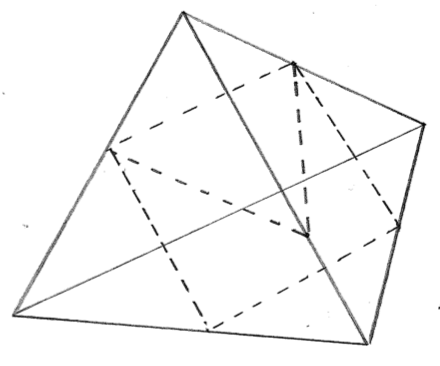
\includegraphics[width=30mm]{./images/finite_element_method_crack_cases_0.png}
  \label{fig:crack_configuration_0}}
    \subfloat[]{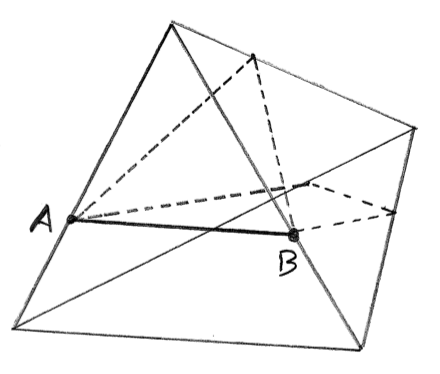
\includegraphics[width=30mm]{./images/finite_element_method_crack_cases_1.png}
  \label{fig:crack_configuration_1}}
    \subfloat[]{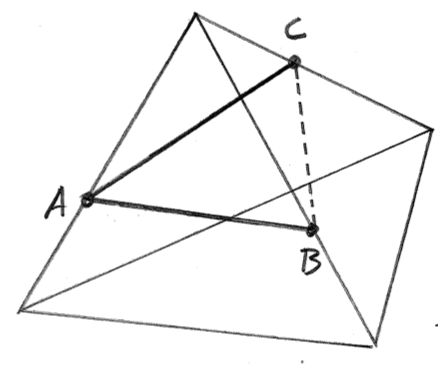
\includegraphics[width=30mm]{./images/finite_element_method_crack_cases_2.png}
  \label{fig:crack_configuration_2}} \\
%\end{center} 
%\begin{center}
    \subfloat[]{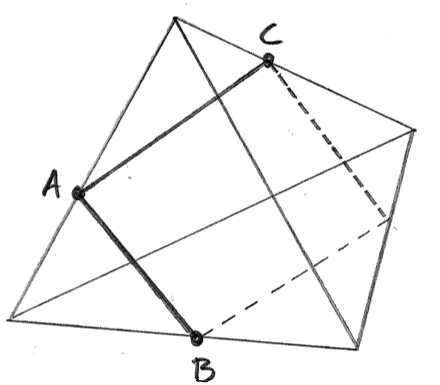
\includegraphics[width=30mm]{./images/finite_element_method_crack_cases_3.png}
  \label{fig:crack_configuration_3}}
    \subfloat[]{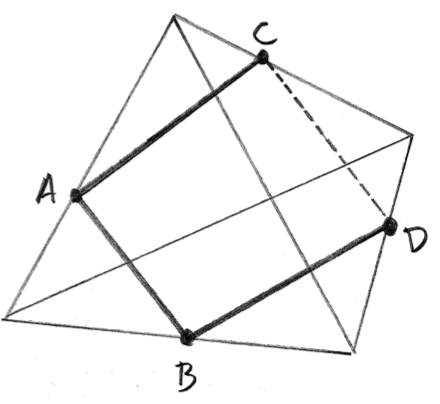
\includegraphics[width=30mm]{./images/finite_element_method_crack_cases_4.png}
  \label{fig:crack_configuration_4}}
    \subfloat[]{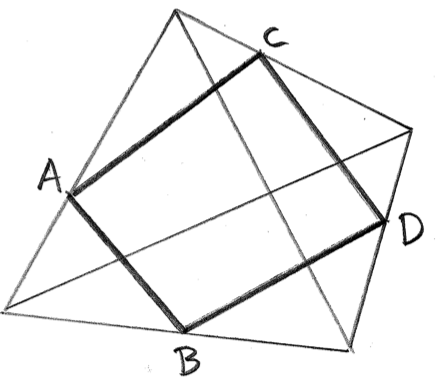
\includegraphics[width=30mm]{./images/finite_element_method_crack_cases_5.png}
  \label{fig:crack_configuration_5}}
 \caption{Crack configurations.}
 \label{fig:crack_configurations}
\end{figure}
%\end{center}

As depicted in figure \vref{fig:crack_configurations} case (a) the
crack plane has no predefined neighbouring edges and is therefore
determined by the maximum principal stress direction alone. When the crack
has been initiated the following crack planes depend on the
element's neighbourhood. Case (b)
illustrates an element about to be 
cracked. In this case the cracked neighbour defines two crack points
that must be located on the crack plane we are about to determine. The
new crack plane is only free to rotate around the edge defined by the
two neighbouring crack points.
The new normal vector $n^{\prime}$ to the plane is determined by the principal stress
direction $n$ and the shared edge defined between crack point $A$ and $B$,
is obtained by:

\begin{equation}
n^{\prime} = n - \biggl[ \frac{n \cdot (A - B)}{|A - B|^2} \biggr] (A - B)
\end{equation}

In case (c-f) the crack plane normal is determined by the pre-existing
neighbouring crack planes. With two or more neighbouring edges the
plane normal is completely determined and the element's maximum
principal stress direction is not considered. Case (a) initiates the
crack which only happens once. From here the crack propagates by
cracking all neighbours in the next iteration, and their neighbours in
the next etc. This way the failure surface will propagate like rings
in the water, from the initial cracked element and out. 